% =====================================================================
% Improving k-Nearest Neighbors on Fashion-MNIST with Learned Distances
% Team report. The author block below is set per team member by
% docs/build_papers.sh (it rewrites \StudentName, \StudentID, \StudentEmail).
% Build all four PDFs from the repository root: bash docs/build_papers.sh
% =====================================================================
\documentclass[10pt,a4paper]{article}

\usepackage[top=1.8cm,bottom=1.8cm,left=1.9cm,right=1.9cm]{geometry}
\usepackage[T1]{fontenc}
\usepackage{lmodern}
\usepackage{microtype}
\usepackage{graphicx}
\usepackage{amsmath,amssymb}
\usepackage{booktabs}
\usepackage{array}
\usepackage{xcolor}
\usepackage{caption}
\usepackage{subcaption}
\usepackage{enumitem}
\usepackage{etoolbox}
\usepackage{placeins}
\usepackage{tikz}
\usetikzlibrary{arrows.meta,positioning}
\usepackage[colorlinks=true,linkcolor=blue!60!black,urlcolor=blue!60!black,citecolor=blue!60!black]{hyperref}
\usepackage{xurl}

\graphicspath{{figures/paper/}}
\captionsetup{font=small,labelfont=bf,skip=4pt}
\setlist{itemsep=0.1em,topsep=0.3em}
% breakable file paths
\newcommand{\file}[1]{\nolinkurl{#1}}
\DeclareMathOperator*{\argmax}{arg\,max}
\DeclareMathOperator*{\argmin}{arg\,min}

% ---- per-student identity (rewritten by docs/build_papers.sh) ----
\newcommand{\StudentName}{Aditi Barman}
\newcommand{\StudentID}{241001001182}
\newcommand{\StudentEmail}{}

\title{\textbf{Improving k-Nearest Neighbors on Fashion-MNIST\\with Learned Distances}\\[0.5em]
\large From 85.2\,\% to 89.5\,\% test accuracy}
\author{\StudentName\\
\small Student ID: \StudentID \quad Batch: BCS 3B\\
\small Techno India University, West Bengal%
\ifdefempty{\StudentEmail}{}{\\ \small\texttt{\StudentEmail}}}
\date{October 2026}

\begin{document}
\maketitle

\begin{center}
\small Team project with Akshar Nath Gorain, Sourodyuti Biswas Sanyal,
Aditi Barman and Sanjana Mahata.\\[3pt]
Code: \href{https://github.com/workforakng/fashion-mnist-knn-optimization}{\nolinkurl{github.com/workforakng/fashion-mnist-knn-optimization}}\\
Demo notebook:
\href{https://colab.research.google.com/github/workforakng/fashion-mnist-knn-optimization/blob/main/fashion_knn_colab.ipynb}{open in Google Colab}
\end{center}

\begin{abstract}
\noindent
The k-nearest neighbors (KNN) classifier labels an image by a vote among the most
similar training images. On Fashion-MNIST, a dataset of clothing images, plain KNN on
raw pixels reaches 85.24\,\% test accuracy. We study how far this can be raised while
the final decision still comes from distances to stored training images. Principal
component analysis (PCA) and a tuned KNN give 86.43\,\%. We then learn the distance
with Soft-KNN, a smooth version of KNN that is close to neighborhood components
analysis. A linear embedding gives 87.10\,\% and a small convolutional network gives
87.63\,\%. The final fusion model (E25) reaches 89.51\,\%. It is not plain KNN. It
mixes a learned neural embedding with neighbor retrieval, ensembling, knowledge
distillation and test-time augmentation. On this test set, single-run differences below
about 0.6 percentage points are within noise. We also report changes that did not
help and the limits of our protocol.
\end{abstract}

% =====================================================================
\section{Introduction}\label{sec:intro}
% =====================================================================
The k-nearest neighbors (KNN) rule~\cite{cover1967} is one of the simplest
classifiers. It has no training step. To label a new image, it finds the $k$ closest
training images and takes a majority vote over their labels.

KNN has two problems on images. First, a $28\times28$ image has $D=784$ pixels. In so
many dimensions, the nearest and the farthest images can be at similar
distances~\cite{beyer1999}. Second, flattening an image into a list of pixels loses
which pixels are next to each other.

Fashion-MNIST~\cite{xiao2017} has 70{,}000 grayscale images of size $28\times28$. They
show ten classes of clothing: T-shirt/top, Trouser, Pullover, Dress, Coat, Sandal,
Shirt, Sneaker, Bag and Ankle boot. There are 60{,}000 training images and
10{,}000 test images. Some classes look alike, such as Shirt, Pullover and Coat.

\textbf{Research question.} How much can we improve KNN on Fashion-MNIST by reducing
the input dimension, by learning the distance, and by combining several models?

\textbf{Approach.} Figure~\ref{fig:pipeline} shows the parts of the final system.
We first tune classical KNN on principal component analysis (PCA) features. We then learn an embedding with
Soft-KNN, a smooth version of KNN that can be trained by gradient descent. A small
convolutional neural network (CNN) gives the best single embedding. We average three such
networks and distill them into one network. The final fusion model (E25) is a weighted
mix of three neighbor-based classifiers.

\begin{figure}[!htb]
\centering
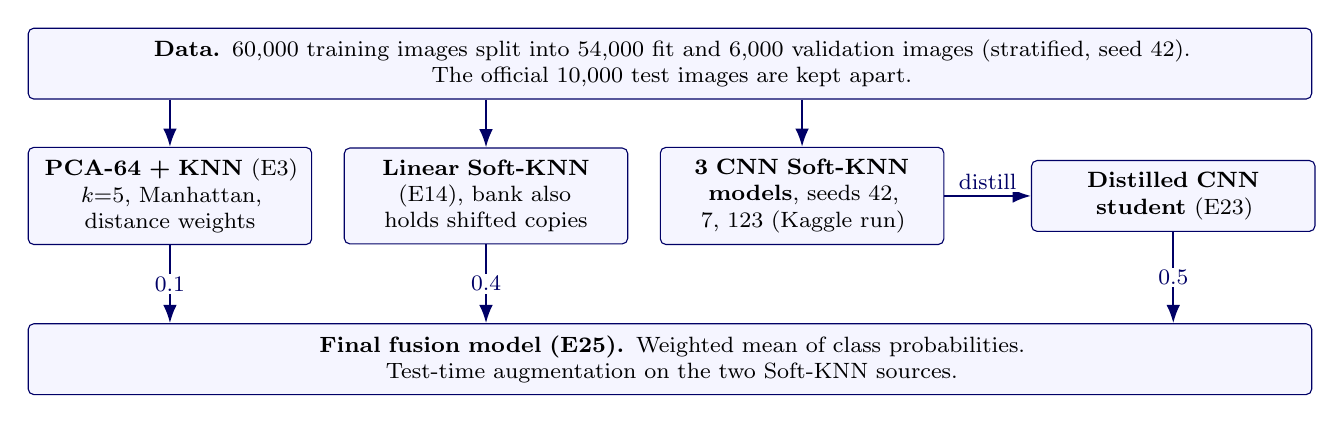
\begin{tikzpicture}[node distance=6mm and 4mm,
  box/.style={draw=blue!40!black, rounded corners=2pt, fill=blue!4,
              inner sep=1.5mm, align=center, font=\footnotesize, text width=3.3cm},
  wide/.style={box, text width=16.0cm},
  arr/.style={-{Latex}, thick, blue!40!black},
  lab/.style={font=\footnotesize, fill=white, inner sep=1pt}]
\node[wide] (data) {\textbf{Data.} 60{,}000 training images split into 54{,}000 fit
  and 6{,}000 validation images (stratified, seed 42).\\ The official 10{,}000 test
  images are kept apart.};
\node[box, below=of data.south west, anchor=north west] (knn)
  {\textbf{PCA-64 + KNN} (E3)\\ $k{=}5$, Manhattan,\\ distance weights};
\node[box, right=of knn] (bank)
  {\textbf{Linear Soft-KNN}\\ (E14), bank also\\ holds shifted copies};
\node[box, right=of bank] (seeds)
  {\textbf{3 CNN Soft-KNN}\\ \textbf{models}, seeds 42,\\ 7, 123 (Kaggle run)};
\node[box, right=11mm of seeds] (student)
  {\textbf{Distilled CNN}\\ \textbf{student} (E23)};
\node[wide, anchor=north] (fusion) at ([yshift=-10mm] data.south |- bank.south)
  {\textbf{Final fusion model (E25).} Weighted mean of class probabilities.\\
  Test-time augmentation on the two Soft-KNN sources.};
\draw[arr] (data.south -| knn) -- (knn);
\draw[arr] (data.south -| bank) -- (bank);
\draw[arr] (data.south -| seeds) -- (seeds);
\draw[arr] (seeds) -- node[lab, above=1pt] {distill} (student);
\draw[arr] (knn) -- node[lab] {0.1} (fusion.north -| knn);
\draw[arr] (bank) -- node[lab] {0.4} (fusion.north -| bank);
\draw[arr] (student) -- node[lab] {0.5} (fusion.north -| student);
\end{tikzpicture}
\caption{Parts of the final fusion model (E25). The numbers on the arrows are the
fusion weights chosen on validation data. The three seed models feed the fusion only
through distillation. Four other candidate sources received weight 0
(Section~\ref{sec:fusion}).}
\label{fig:pipeline}
\end{figure}

\textbf{Contributions.}
\begin{itemize}[leftmargin=1.4em]
\item A study of classical KNN on Fashion-MNIST: distance measures, PCA, the choice
      of $k$ and query time (Section~\ref{sec:classical}).
\item A Soft-KNN model that learns the distance over a memory bank of training images.
      It follows neighborhood components analysis~\cite{goldberger2004} and its
      scalable version~\cite{wu2018snca}. We do not claim it is new
      (Section~\ref{sec:softknn}).
\item A convolutional embedding, a seed ensemble, distillation and a weighted fusion
      that reach 89.51\,\% test accuracy (Section~\ref{sec:conv}).
\item A list of changes that did not help (Section~\ref{sec:negative}) and the limits
      of our protocol (Section~\ref{sec:limits}).
\end{itemize}

Every run is logged in a JSON (JavaScript Object Notation) file in the repository (the \emph{ledger},
\file{results/results.json}). We name runs by their ledger ID, such as E1 or E25.
Section~\ref{sec:main} summarizes the main runs.

% =====================================================================
\section{Related Work}\label{sec:related}
% =====================================================================
Cover and Hart~\cite{cover1967} showed that the error of the nearest-neighbor rule is
at most twice the best possible error, given unlimited data. Beyer et
al.~\cite{beyer1999} showed that in high dimensions, distances to the nearest and the
farthest point can become nearly equal.

Several methods learn a distance for KNN. Neighborhood components analysis
(NCA)~\cite{goldberger2004} learns a linear map. It trains a soft version of the
leave-one-out KNN error over all training points. Large margin nearest neighbor
(LMNN)~\cite{weinberger2009} learns a distance that keeps same-class neighbors close
and pushes other classes away.

Wu et al.~\cite{wu2018unsup} store the embeddings of all training images in a
\emph{memory bank}. The bank is updated during training, so the network does not
recompute every embedding at every step. Wu, Efros and Yu~\cite{wu2018snca} combine
such a bank with an NCA loss and a deep network, and they classify by KNN. Our
Soft-KNN is close to this scalable NCA.

Knowledge distillation~\cite{hinton2015} trains a \emph{student} network to match
the class probabilities of a \emph{teacher} network. We tune classical KNN with
Optuna~\cite{akiba2019}, a library for hyperparameter search.

% =====================================================================
\section{Data and Protocol}\label{sec:protocol}
% =====================================================================
\textbf{Splits.} We split the 60{,}000 training images into 54{,}000 \emph{fit}
images and 6{,}000 \emph{validation} images. The split keeps the class balance
(stratified, seed 42). The official 10{,}000 test images are used only to report
results. Pixels are scaled to $[0,1]$.

\textbf{Rules.} We choose models and settings by validation accuracy. We compute test
accuracy after each choice, but no setting is chosen by test accuracy. The global
seed is 42, except in the seed study.

\textbf{Uncertainty.} We write differences in percentage points (pp). On 10{,}000 test
images, one binomial standard error (SE) of accuracy is about $\pm0.3$\,pp. So a gap
under about 0.6\,pp between two single runs is not reliable. We mark such gaps as
``within noise''. On the 6{,}000 validation images, one SE is about 0.4\,pp. We ran
no significance tests.

\textbf{Validation reuse.} We used the same 6{,}000 validation images for many
choices. These include the PCA dimension, the Optuna search, early stopping, the
inference settings and the fusion weights. So the best validation accuracy
(90.85\,\%) is optimistic. The test accuracy is the fair estimate.

\textbf{Where the runs ran.} The stages in \file{src/experiments.py} ran on the
authors' local machine. The distilled student (E23) and its three teacher models
were trained on Kaggle graphics processing units (GPUs)
(\file{results/kaggle_*.json}). The seed models in
E21 come from a separate run of the same seed script
(\file{results/conv_seeds.json}).

% =====================================================================
\section{Classical KNN Baselines}\label{sec:classical}
% =====================================================================
\subsection{Distance Measures on Raw Pixels}\label{sec:metrics}
For two images $x, x' \in [0,1]^{D}$, we compare three distances:
\begin{equation}
\delta_2(x,x') = \lVert x-x'\rVert_2, \qquad
\delta_1(x,x') = \textstyle\sum_{j=1}^{D}|x_j-x'_j|, \qquad
\delta_{\cos}(x,x') = 1-\dfrac{x^\top x'}{\lVert x\rVert_2\,\lVert x'\rVert_2}.
\end{equation}
Here $\delta_2$ is the Euclidean distance, $\delta_1$ the Manhattan distance and
$\delta_{\cos}$ the cosine distance. KNN predicts
$\hat{y}(x)=\argmax_{c}\sum_{i\in\mathcal{N}_k(x)}\mathbb{1}[y_i=c]$. Here
$\mathcal{N}_k(x)$ holds the $k$ nearest fit images, and $y_i$ is the label of fit image
$i$. The indicator $\mathbb{1}[\cdot]$ is 1 if its condition holds and 0 otherwise. The
class $c$ is one of $C=10$ classes.

Table~\ref{tab:metrics} shows raw-pixel KNN with $k=5$ and equal votes. The
Euclidean run is ledger entry E1. The Manhattan and cosine runs come from a later
logged rerun (\file{results/classical_reruns.json}). Manhattan is the most
accurate, at 85.91\,\% test accuracy (+0.67\,pp over Euclidean). Cosine is +0.39\,pp
over Euclidean, which is within noise. We did not test why Manhattan does better.

\begin{table}[!htb]
\centering\small
\caption{KNN on raw 784-pixel inputs ($k=5$, equal votes). Val and Test are
accuracies in \%. Macro F1 is the mean F1 score over the ten classes. Time is the
median of 3 runs for 10{,}000 test queries on a 4-core Intel Xeon (2.10\,GHz).}
\label{tab:metrics}
\begin{tabular}{llcccc}
\toprule
ID & Distance & Val (\%) & Test (\%) & Macro F1 & Time (s) \\
\midrule
E1 & Euclidean & 86.13 & 85.24 & 0.8518 & 4.64 \\
--- & Manhattan & 86.97 & 85.91 & 0.8583 & 84.00 \\
--- & Cosine    & 86.18 & 85.63 & 0.8543 & 10.75 \\
\bottomrule
\end{tabular}
\end{table}

\subsection{Reducing the Dimension with PCA}\label{sec:pca}
PCA~\cite{jolliffe2016} keeps the $d$ directions in
which the fit images vary most. We fit PCA on the 54{,}000 fit images only.
Figure~\ref{fig:pca}(a) shows that $d=64$ components keep 88.1\,\% of the variance.
The 90\,\% level is first reached at $d=84$.

Figure~\ref{fig:pca}(b) shows the validation accuracy of KNN ($k=5$, Euclidean) on
PCA features. The best value is at $d=64$ (87.33\,\%). Beyond $d=48$ the curve is
flat within noise. On test data, PCA-64 with the same KNN gives 85.63\,\%. That is
+0.39\,pp over raw pixels, which is within noise.

\begin{figure}[!htb]
\centering
\begin{subfigure}[t]{0.48\textwidth}
\centering
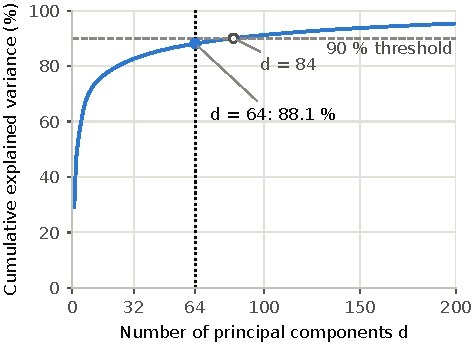
\includegraphics[width=\linewidth]{pca_variance.pdf}
\caption{Cumulative explained variance.}
\end{subfigure}\hfill
\begin{subfigure}[t]{0.48\textwidth}
\centering
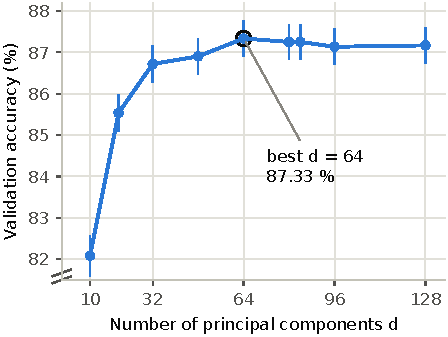
\includegraphics[width=\linewidth]{pca_sweep.pdf}
\caption{Validation accuracy versus $d$.}
\end{subfigure}
\caption{(a) Cumulative variance explained by PCA fitted on the 54{,}000 fit images.
The dotted line marks $d=64$ (88.1\,\%). The dashed line marks 90\,\%, first reached
at $d=84$. (b) Validation accuracy of KNN ($k=5$, Euclidean) on PCA features (E2).
The best value is at $d=64$ (87.33\,\%), and the curve is flat beyond $d=48$. Bars
show $\pm1$ SE.}
\label{fig:pca}
\end{figure}

\subsection{\texorpdfstring{Choosing $k$ and Tuning KNN}{Choosing k and Tuning KNN}}\label{sec:biasvar}
A small $k$ follows the fit images closely and is sensitive to noise. A large $k$
gives smoother decisions but can mix neighboring classes. Figure~\ref{fig:biasvar}
shows a sweep over $k=1,3,\dots,25$ on PCA-64 features (E4). Validation accuracy
peaks at $k=7$ (87.37\,\%). The values for $k=5$, 7 and 9 are within noise.


We then tuned KNN on PCA-64 features with Optuna~\cite{akiba2019} for 40 trials (E3).
The search covered $k$, the vote weights and the distance measure. The PCA dimension
stayed fixed at 64. The best setting was $k=5$, Manhattan distance, and votes weighted
by inverse distance. Inverse-distance weights give closer neighbors more say. This
model reaches 87.82\,\% validation and 86.43\,\% test accuracy (E3). That is
+1.19\,pp over raw-pixel KNN. On raw pixels, the Manhattan distance alone already
gives 85.91\,\% (Table~\ref{tab:metrics}).

\subsection{Query Time}\label{sec:latency}
Brute-force KNN compares each query with all 54{,}000 fit images. Its cost grows with
the number of dimensions. Figure~\ref{fig:latency} shows the timing run in the ledger
(E5). It timed all 6{,}000 validation queries in one call. Brute-force search took
2.98\,s on raw pixels and 0.418\,s on PCA-64 features, a $7.12\times$ speed-up. The
tree-based searches were slower than brute force.

\begin{figure}[!htb]
\centering
\begin{minipage}[t]{0.48\textwidth}
\centering
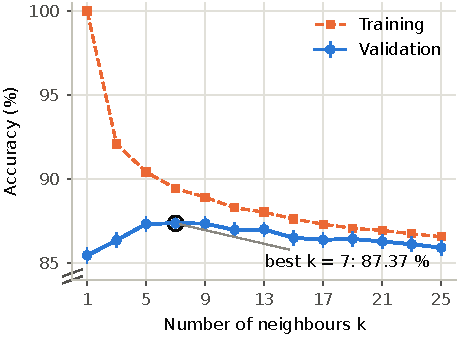
\includegraphics[width=\linewidth]{bias_variance.pdf}
\caption{Training and validation accuracy of PCA-64 KNN (equal votes) for
$k=1$--25 (E4). Validation accuracy peaks at $k=7$, but $k=5$--9 are within noise.
Training accuracy at $k=1$ is 100\,\% because each training point is its own
neighbor. Bars show $\pm1$ SE.}
\label{fig:biasvar}
\end{minipage}\hfill
\begin{minipage}[t]{0.48\textwidth}
\centering
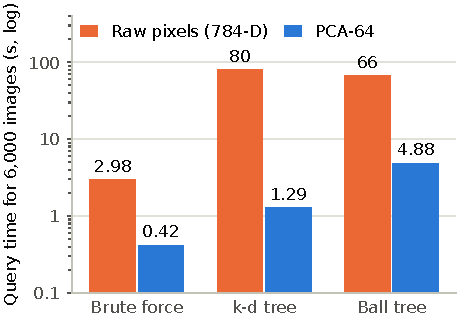
\includegraphics[width=\linewidth]{latency.pdf}
\caption{Query time of KNN for the 6{,}000 validation images on raw pixels and on
PCA-64 features (E5, log scale, Euclidean distance). Brute force is the median of 3
runs. The k-d tree and ball tree were timed once and are slower than brute force.}
\label{fig:latency}
\end{minipage}
\end{figure}

We repeated the timing with a fixed protocol (\file{results/classical_reruns.json}).
It used the 10{,}000 test queries, a 4-core Intel Xeon, one warm-up run and the median
of 3 runs. Raw pixels took 4.64\,s and PCA-64 took 1.49\,s, a $3.1\times$ speed-up.
So the size of the speed-up depends on the hardware. The speed-up also does not hold
for the tuned model. It uses the Manhattan distance and took 15.73\,s, which is
slower than raw-pixel Euclidean KNN.

% =====================================================================
\section{Soft-KNN: Learning the Distance}\label{sec:softknn}
% =====================================================================
\subsection{Model}\label{sec:softknn-model}
A majority vote does not change smoothly when the features change. So gradient
descent cannot learn a better distance through it. Soft-KNN replaces the vote with a
smooth score, as in NCA~\cite{goldberger2004}.

An embedding network $f_\theta$ maps an image $x$ to a vector. Here $\theta$ are the
network weights. We use the unit-length embedding $z=f_\theta(x)/\lVert
f_\theta(x)\rVert_2\in\mathbb{R}^{128}$. The simplest $f_\theta$ is a linear map
$f_\theta(x)=Wx$, with a $128\times784$ matrix $W$.

A \emph{memory bank} stores the embeddings $b_1,\dots,b_N$ of all $N=54{,}000$ fit
images, with labels $y_1,\dots,y_N$. For each class $c$, let $\mathcal{A}_c(x)$ be
the $m$ bank entries of class $c$ that are closest to $z$. Note that $m$ counts
neighbors \emph{per class} (the code calls it $k$). The mean distance to class $c$ is
\begin{equation}
\bar\delta_c(x)=\frac{1}{m}\sum_{i\in\mathcal{A}_c(x)}\lVert z-b_i\rVert_2 .
\end{equation}
The model turns these distances into class probabilities with a temperature $\tau>0$:
\begin{equation}
P_\tau(y=c\mid x)=\frac{\exp\!\left(-\bar\delta_c(x)/\tau\right)}
{\sum_{c'=1}^{C}\exp\!\left(-\bar\delta_{c'}(x)/\tau\right)} .
\label{eq:softknn}
\end{equation}
Training minimizes the cross-entropy (CE) loss $-\log P_\tau(y\mid x)$ over the fit
images.

\textbf{What the model predicts.} For every $\tau>0$, the predicted class is
$\argmin_c\bar\delta_c(x)$. This is the class whose $m$ nearest members are closest on
average. It is a local-mean rule~\cite{mitani2006}, not a majority vote. The
temperature $\tau$ does not change the predicted class at test time. It only changes
how confident the probabilities are. It also changes training, because the loss
depends on these probabilities. The logged inference grids confirm this: in E19, the
validation accuracy for each $m$ is the same for $\tau=0.1$, 0.3 and 0.5.

\textbf{What is trained.} Gradients flow only through the selected distances
$\lVert z-b_i\rVert_2$ into the query embedding $z$. Choosing the $m$ nearest entries
is not differentiable. The bank is detached, so no gradient reaches the stored
embeddings $b_i$.

\textbf{Memory bank.} Recomputing all 54{,}000 bank embeddings after every step would
be slow. So we refresh the bank at fixed times, as in Wu et al.~\cite{wu2018unsup,
wu2018snca}. The linear models refresh once per epoch (211 steps of 256 images). The
MLP and convolutional models refresh every 107 steps. Unlike momentum contrast (MoCo)~\cite{he2020},
there is no second, slowly updated encoder.

\textbf{Self-match.} Training images are also in the bank. So a training query finds
its own (slightly older) embedding at a distance near zero. This inflates training
accuracy and changes the training loss. Validation and test images are never in the
bank. The code now has an opt-in fix (\texttt{-{}-exclude-self}), but all logged
numbers were produced without it.

\subsection{Linear, MLP and Bank-Augmented Embeddings}\label{sec:linear}
The linear model (E6) maps 784 pixels to 128 numbers. Its matrix $W$ starts from the
PCA directions. We train it with Adam~\cite{kingma2015} (learning rate $10^{-3}$,
batch size 256, $m=7$, $\tau=0.5$). It reaches 88.22\,\% validation and 87.10\,\%
test accuracy. That is +0.67\,pp over the tuned classical KNN (E3).

A multilayer perceptron (MLP) with layers 784--256--128 did worse (E16, 85.70\,\%
test). It used Adam with learning rate $3\times10^{-4}$ and gradient clipping.

In E14 the bank also holds a shifted copy of each fit image (shift of up to 2 pixels).
The queries stay unchanged. This gives 87.13\,\% test, +0.03\,pp over E6, which is
within noise. We still use this model, because the fusion gives it a large weight.

\subsection{Temperature}\label{sec:tau}
We trained the linear model with six values of $\tau$ from 0.1 to 1.0 (E8).
Figure~\ref{fig:tau} shows that validation accuracy falls as $\tau$ grows. The best
tested value is $\tau=0.1$ (86.53\,\%), at the edge of the grid. We did not test
smaller values. These models were trained with flip, shift and erase augmentation and
at most 10 epochs. They were all scored at $\tau=0.5$. The scoring $\tau$ does not affect accuracy.

One possible reason for the trend: the embeddings have unit length, so each
$\bar\delta_c$ lies in $[0,2]$. At $\tau=1$, no class can then get more than
$1/(1+9e^{-2})\approx45\,\%$ probability. So the loss stays high even for correct
predictions. We did not test this explanation. The value chosen in E8 was not used for
training later models. The CNN models were trained at $\tau=0.5$ and scored at
$\tau=0.1$.


\subsection{Optimizer Pilot}\label{sec:optim}
We compared three optimizers on the linear model (E9), with the same short,
augmented schedule as E8. Stochastic gradient descent (SGD) used plain momentum 0.9
(not Nesterov) and learning rate 0.1. Adam~\cite{kingma2015} and RMSprop~\cite{tieleman2012} used
learning rate $10^{-3}$. RMSprop scales each step by a running mean of squared
gradients, which is a second moment.

Figure~\ref{fig:optim} shows the results. SGD was best: 83.85\,\% validation accuracy
during training and 86.22\,\% after re-scoring. Adam reached 81.47\,\% and 82.50\,\%.
RMSprop reached 80.83\,\% and 82.72\,\%. The learning rates differ by a factor of 100,
and each optimizer ran once. So this is a small pilot, not a fair comparison. All
later models still used Adam.

\begin{figure}[!htb]
\centering
\begin{minipage}[t]{0.48\textwidth}
\centering
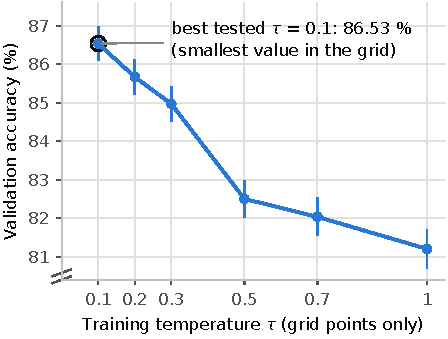
\includegraphics[width=\linewidth]{tau_sweep.pdf}
\caption{Validation accuracy of the linear Soft-KNN trained with each $\tau$ (E8).
Only the six marked values were tested. Accuracy falls as $\tau$ grows. The best
tested value, $\tau=0.1$, is the smallest in the grid. Bars show $\pm1$ SE.}
\label{fig:tau}
\end{minipage}\hfill
\begin{minipage}[t]{0.48\textwidth}
\centering
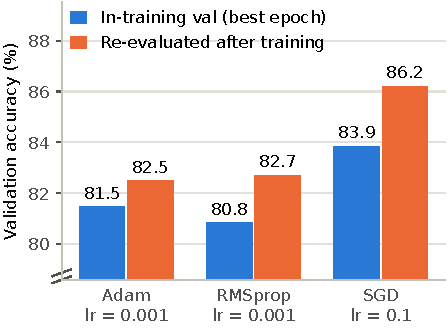
\includegraphics[width=\linewidth]{optimizer.pdf}
\caption{Optimizer pilot (E9) on the linear Soft-KNN with augmentation and at most
10 epochs. Blue: best validation accuracy during training. Orange: the returned model
scored again with a fresh bank. Learning rates differ.}
\label{fig:optim}
\end{minipage}
\end{figure}

% =====================================================================
\section{Convolutional Embedding, Ensembles and Fusion}\label{sec:conv}
% =====================================================================
\subsection{Convolutional Embedding}\label{sec:convmodel}
A linear map ignores which pixels are neighbors. So we replace $W$ with a small CNN.
It has two blocks of $3\times3$ convolution, rectified linear unit (ReLU) and
$2\times2$ max-pooling, with 32 and 64 channels. A linear layer then maps the
$64\times7\times7$ features to 128 numbers, which we scale to unit length.

The first CNN run (E19, seed 42) used Adam with learning rate $3\times10^{-4}$,
gradient clipping at 1.0 and batch size 256. It trained for the full 30 epochs.
Early stopping, with a patience of 8 epochs, did not trigger. At inference we use $m=9$ and
$\tau=0.1$. It reaches 89.07\,\% validation and 87.63\,\% test accuracy, +0.53\,pp
over the linear model.

\subsection{Seed Ensemble}\label{sec:ensemble}
We trained the same CNN with seeds $s\in\mathcal{S}=\{42,7,123\}$. These runs used
automatic mixed precision (AMP), up to 35 epochs and a patience of 10 epochs. Seed 123
stopped after 14 epochs. The ensemble averages the class probabilities:
$\bar{P}(y=c\mid x)=\frac{1}{3}\sum_{s\in\mathcal{S}}P^{(s)}(y=c\mid x)$. Here
$P^{(s)}$ is the output of the model trained with seed $s$.

Figure~\ref{fig:seeds} shows the three seeds and their ensemble (E21). The test
accuracies are 87.53\,\%, 86.92\,\% and 87.57\,\%. Their mean is 87.34\,\% with a
standard deviation of 0.36\,pp. The ensemble reaches 88.06\,\%. That is +0.49\,pp over
the best seed, which is within noise, and +0.72\,pp over the seed mean. The ensemble
needs three networks at test time.

\begin{figure}[!htb]
\centering
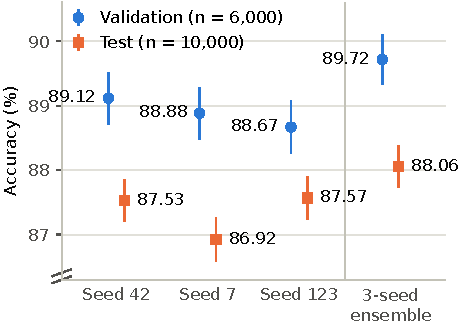
\includegraphics[width=0.48\textwidth]{seeds.pdf}
\caption{Validation and test accuracy of the three CNN seed models and of their
ensemble (E21). Bars show $\pm1$ SE. The seed spread on test is 0.65\,pp.}
\label{fig:seeds}
\end{figure}

\subsection{Knowledge Distillation}\label{sec:distill}
Distillation~\cite{hinton2015} trains one student network to copy a teacher. Our
teacher is the mean of three CNN seed models. For each fit image $x_i$, the teacher
gives class probabilities $p^{\mathrm{T}}(x_i)$, computed with Soft-KNN at $m=9$ and
$\tau=1$. The student is a new CNN with Soft-KNN scores
$h_c(x)=-\bar\delta_c(x)/\tau$ (training $\tau=0.5$). It minimizes
\begin{equation}
\mathcal{L}=(1-\lambda)\,\mathrm{CE}\big(y,\operatorname{softmax}(h)\big)
+\lambda\,T^{2}\,\mathrm{KL}\big(p^{\mathrm{T}}\,\big\Vert\,\operatorname{softmax}(h/T)\big).
\end{equation}
Here KL is the Kullback--Leibler divergence, $\lambda=0.5$ weights the two terms and
$T=1$ is the distillation temperature. With $T=1$ the second term is simply
$\mathrm{KL}(p^{\mathrm{T}}\Vert P_\tau)$.

The student and its three teacher models were trained on Kaggle. The teachers
are a separate run of seeds 42, 7 and 123, with test accuracies 87.44\,\%, 87.25\,\%
and 87.54\,\%. The student uses the same settings as the seed models.

The student (E23) reaches 90.10\,\% validation and 89.03\,\% test accuracy. That is
+1.49\,pp over its best teacher model and +0.97\,pp over the E21 ensemble. This is a
single run, and we do not claim a cause. A second Kaggle student, trained with five
teacher seeds, reached 89.01\,\%. It is not used in any fusion.

Two caveats apply to the teacher targets. First, the teacher scored fit images that
are in its own bank. Each image matched itself, so the targets partly encode the true
labels. Second, at $\tau=1$ the targets are far from one-hot. As shown above, no class
can get more than about 45\,\%. So the targets act partly like smoothed labels.

\subsection{Test-Time Augmentation and Fusion}\label{sec:fusion}
Test-time augmentation (TTA) averages a model's predictions over six versions of each
query: the original, a horizontal flip and four 1-pixel shifts. We apply it to the
Soft-KNN sources in the last fusion.

The fusion combines $J$ sources with weights:
$P(y=c\mid x)=\sum_{j=1}^{J}w_jP_j(y=c\mid x)$, with $w_j\ge0$ and $\sum_jw_j=1$. We
try all weight vectors on a grid with step 0.1. For the seven sources of E24 and E25,
that is 8{,}008 vectors. We keep the vector with the best validation accuracy.

Table~\ref{tab:fusion} lists the sources and weights. E22 fused six sources. E24 added
the distilled student and reached 89.36\,\%. E25 added TTA and searched the weights
again. It reached 89.51\,\% test and 90.85\,\% validation accuracy. The gain of E25
over E24 is +0.15\,pp, which is within noise. Only three sources have nonzero weight in
E25: the bank-augmented linear model (0.4), PCA-64 KNN (0.1) and the student (0.5).

\begin{table}[!htb]
\centering\small
\caption{Fusion sources and the weights chosen on validation data (grid step 0.1).
Soft-KNN sources use $\tau=0.1$. TTA is used only in E25.}
\label{tab:fusion}
\begin{tabular}{llccc}
\toprule
Source & Inference setting & E22 & E24 & E25 \\
\midrule
CNN seed 42           & $m=9$ & 0.2 & 0.2 & 0.0 \\
CNN seed 7            & $m=9$ & 0.2 & 0.0 & 0.0 \\
CNN seed 123          & $m=9$ & 0.1 & 0.0 & 0.0 \\
Linear Soft-KNN, bank-augmented (E14) & $m=5$ & 0.4 & 0.4 & 0.4 \\
MLP Soft-KNN (E16)    & $m=9$ & 0.0 & 0.0 & 0.0 \\
PCA-64 KNN (E3)       & $k=5$ & 0.1 & 0.1 & 0.1 \\
Distilled student (E23) & $m=9$ & --- & 0.3 & 0.5 \\
\midrule
Validation accuracy (\%) & & 90.27 & 90.62 & 90.85 \\
Test accuracy (\%)       & & 88.73 & 89.36 & 89.51 \\
\bottomrule
\end{tabular}
\end{table}

% =====================================================================
\section{Results}\label{sec:results}
% =====================================================================
\subsection{Main Results}\label{sec:main}
Table~\ref{tab:main} lists the main runs. The rows are grouped by method, not by the
order in which they ran. The ledger also holds earlier fusions (E11, E15, E17) and
diagnostic runs, which we leave out here.

\begin{table}[!htb]
\centering\small
\caption{Main results on Fashion-MNIST. Val and Test are accuracies in \% on 6{,}000
validation and 10{,}000 test images. ``---'' means the value was not logged. Rows
without an ID, and the values marked $^\dagger$, come from the logged rerun of
classical KNN.}
\label{tab:main}
\begin{tabular}{@{}l>{\raggedright\arraybackslash}p{0.52\textwidth}ccc@{}}
\toprule
ID & Method & Val (\%) & Test (\%) & Macro F1 \\
\midrule
E1  & KNN, raw pixels, Euclidean, $k=5$ & 86.13 & 85.24 & 0.8518 \\
--- & KNN, raw pixels, Manhattan, $k=5$ & 86.97 & 85.91 & 0.8583 \\
E2  & KNN, PCA-64, Euclidean, $k=5$ & 87.33 & 85.63$^\dagger$ & 0.8557$^\dagger$ \\
E3  & KNN, PCA-64, tuned with Optuna (Manhattan, $k=5$, distance weights) & 87.82 & 86.43 & 0.8644 \\
\midrule
E6  & Soft-KNN, linear embedding & 88.22 & 87.10 & 0.8698 \\
E14 & Soft-KNN, linear, bank with shifted copies & 88.28 & 87.13 & 0.8703 \\
E16 & Soft-KNN, MLP embedding & 86.92 & 85.70 & --- \\
\midrule
E19 & Soft-KNN, CNN embedding (seed 42) & 89.07 & 87.63 & --- \\
E21 & Ensemble of three CNN seed models & 89.72 & 88.06 & --- \\
E23 & Distilled CNN student & 90.10 & 89.03 & --- \\
\midrule
E22 & Fusion of six sources & 90.27 & 88.73 & 0.8858 \\
E24 & Fusion of seven sources & 90.62 & 89.36 & 0.8923 \\
E25 & \textbf{Final fusion model}: seven sources with TTA & \textbf{90.85} & \textbf{89.51} & \textbf{0.8936} \\
\bottomrule
\end{tabular}
\end{table}

The final fusion model (E25) is +4.27\,pp above raw-pixel KNN (E1). It is +0.48\,pp
above the best single model, the distilled student (E23). That gap is within noise.
The largest steps were tuning classical KNN (+1.19\,pp, E1 to E3) and distillation
(+0.97\,pp over the E21 ensemble).

The gap between validation and test accuracy is 1.34\,pp for E25. It is 1.44\,pp for
the single CNN model E19. So the fusion search did not add a large extra gap.

Figure~\ref{fig:cm} shows the errors of E25. Recall is highest for Bag (98.5\,\%),
Trouser (97.9\,\%) and Sneaker (97.0\,\%). Shirt is lowest at 61.7\,\%. Of all shirts,
16\,\% are predicted as T-shirt/top. Most other errors are among Pullover, Coat and
Shirt. The matrix is not stored in the ledger. Its counts were read from the E25 output
figure, and their diagonal matches the logged 89.51\,\%.

\begin{figure}[!htbp]
\centering
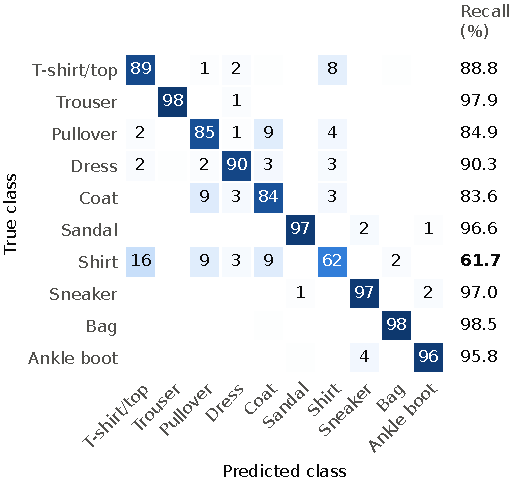
\includegraphics[width=0.5\textwidth]{confusion_matrix.pdf}
\caption{Row-normalized confusion matrix (\%) of the final fusion model (E25) on the
10{,}000 test images. The last column is per-class recall. Recall is highest for Bag
(98.5\,\%), Trouser (97.9\,\%) and Sneaker (97.0\,\%). Shirt is lowest (61.7\,\%), and
16\,\% of shirts are predicted as T-shirt/top.}
\label{fig:cm}
\end{figure}

\subsection{Changes That Did Not Help}\label{sec:negative}
Table~\ref{tab:negative} lists changes that did not improve test accuracy.

\begin{table}[!htb]
\centering\small
\caption{Changes that did not improve test accuracy. $\Delta$ is the difference in pp
to the reference run. Gaps under about 0.6\,pp are within noise.}
\label{tab:negative}
\begin{tabular}{@{}l>{\raggedright\arraybackslash}p{0.5\textwidth}ccc@{}}
\toprule
ID & Change & Test (\%) & Reference & $\Delta$ (pp) \\
\midrule
E7  & Flip, shift and erase on training queries (linear) & 81.68 & E6 & $-5.42$ \\
E13 & Shift on training queries (linear) & 83.66 & E6 & $-3.44$ \\
E20 & Shift on training queries (CNN) & 84.62 & E19 & $-3.01$ \\
E26 & Second round of distillation & 87.00 & E23 & $-2.03$ \\
E16 & MLP instead of linear embedding & 85.70 & E6 & $-1.40$ \\
E10 & TTA on the linear model & 86.74 & E6 & $-0.36$ \\
E14 & Shifted copies in the bank only & 87.13 & E6 & $+0.03$ \\
\bottomrule
\end{tabular}
\end{table}

Augmenting the training queries hurt in all three runs (E7, E13, E20). These runs
were short, used one seed, and in E7 combined three changes. So they do not show that
augmentation is harmful in general. One possible factor is self-match. Clean queries
can match themselves in the bank, but augmented queries cannot.

TTA lowered the linear model from 87.10\,\% to 86.74\,\% (E10). This is within
noise. On the augmented model of E7, TTA raised test accuracy from 81.68\,\% to
82.60\,\%. In E25, TTA was added together with a new weight search, so its own effect is
unknown.

The second round of distillation (E26) used the E24 fusion as teacher, not the first
student alone. Its teacher weights were 0.2 for CNN seed 42, 0.4 for the bank-augmented
model, 0.1 for PCA-64 KNN and 0.3 for the student. The teacher again scored fit images
that were in its own banks. Its KNN part even returns the true label exactly, because
each fit image is its own nearest neighbor at distance zero. The new student reached
87.00\,\%, which is 2.03\,pp below the first student. The teacher changed in several
ways at once, so we cannot say why.

\FloatBarrier
% =====================================================================
\section{Limitations}\label{sec:limits}
% =====================================================================
\begin{itemize}[leftmargin=1.4em]
\item \textbf{Self-match.} Training queries and teacher targets were computed with
      each image in its own bank. The opt-in \texttt{-{}-exclude-self} fix was not used
      for any logged number.
\item \textbf{Validation reuse.} The same validation images chose many settings, so
      validation accuracies are optimistic. Some inference settings ($m=9$ for the CNN
      models, $m=5$ for the bank-augmented model) were fixed by hand.
\item \textbf{Stale bank.} Early stopping scored validation images against the bank
      from the last refresh, not against fresh embeddings.
\item \textbf{Noise.} Most results are single runs. We ran no significance tests, and
      the CNN seeds alone differ by up to 0.65\,pp.
\item \textbf{Missing controls.} We did not test a hard KNN vote on the learned
      embedding. We did not train the same CNN with a standard classification layer.
      So we cannot say whether the neighbor-based output helps.
\item \textbf{Scope.} We used one dataset. The final accuracy is in the range of the
      classical baselines reported with the dataset~\cite{xiao2017}, such as support
      vector machines.
\item \textbf{Mixed environments.} Some models were trained on Kaggle, and AMP makes
      GPU runs not exactly repeatable. The same seeds gave different accuracies in two
      runs (\file{results/conv_seeds.json} and \file{results/kaggle_conv_seeds.json}).
\item \textbf{Notebook.} The Colab notebook is a simplified demo. It does not
      reproduce the reported numbers (Section~\ref{sec:repro}).
\end{itemize}

% =====================================================================
\section{Conclusion and Future Work}\label{sec:conclusion}
% =====================================================================
We raised test accuracy on Fashion-MNIST from 85.24\,\% (raw-pixel KNN) to
89.51\,\% (the final fusion model, E25). Tuning classical KNN on PCA features gave
86.43\,\%. Learning the distance with Soft-KNN gave 87.10\,\% with a linear embedding
and 87.63\,\% with a CNN. Ensembling, distillation and fusion gave the rest. Every
model still decides from distances to stored training images. However, the final
system depends on a trained neural embedding and on several combined models.

Future work should rerun the learned models with self-match excluded and with
several seeds. It should add the missing controls, use a separate split for the
fusion weights, and test other embedding sizes.

% =====================================================================
\section{Reproducibility}\label{sec:repro}
% =====================================================================
The code, the ledger and the figures are in the
\href{https://github.com/workforakng/fashion-mnist-knn-optimization}{GitHub repository}
linked on the title page.
All reported numbers come from the following commands:
\begin{itemize}[leftmargin=1.4em]
\item \texttt{python -m src.experiments -{}-scale full -{}-stages E1,E2,...} runs the
      ledger stages and appends to \file{results/results.json}.
\item \texttt{python scripts/train\_conv\_seed.py -{}-seed 42} and
      \texttt{python scripts/train\_distill.py} train the seed models and the student.
\item \texttt{python scripts/rerun\_classical.py} repeats the classical KNN runs and
      timings.
\item \texttt{python scripts/make\_paper\_figures.py} draws the figures, and
      \texttt{bash docs/build\_papers.sh} builds this report.
\end{itemize}
Trained models are not stored in the repository. So the stages from E10 on need the
models to be trained again. The fusion stages use whichever trained models exist, so
a rerun may use other sources than the logged run.

The \href{https://colab.research.google.com/github/workforakng/fashion-mnist-knn-optimization/blob/main/fashion_knn_colab.ipynb}{Colab
notebook} is a short teaching demo. It runs classical KNN on a subset of the images
and a small CNN with learned class prototypes. It has no memory bank, ensemble,
distillation or fusion, and it does not reproduce the numbers in this report.

% =====================================================================
\footnotesize
\begin{thebibliography}{99}
\setlength{\itemsep}{0pt}
\bibitem{cover1967} T.~M. Cover and P.~E. Hart. Nearest neighbor pattern
classification. \emph{IEEE Transactions on Information Theory}, 13(1):21--27, 1967.
\bibitem{beyer1999} K.~Beyer, J.~Goldstein, R.~Ramakrishnan, and U.~Shaft. When is
``nearest neighbor'' meaningful? In \emph{Proc.\ International Conference on Database
Theory (ICDT)}, LNCS 1540, pages 217--235. Springer, 1999.
\bibitem{xiao2017} H.~Xiao, K.~Rasul, and R.~Vollgraf. Fashion-MNIST: A novel image
dataset for benchmarking machine learning algorithms. arXiv preprint
arXiv:1708.07747, 2017.
\bibitem{goldberger2004} J.~Goldberger, S.~Roweis, G.~Hinton, and
R.~Salakhutdinov. Neighbourhood components analysis. In \emph{Advances in Neural
Information Processing Systems 17 (NIPS 2004)}, pages 513--520, 2004.
\bibitem{wu2018snca} Z.~Wu, A.~A. Efros, and S.~X. Yu. Improving generalization via
scalable neighborhood component analysis. In \emph{Proc.\ European Conference on
Computer Vision (ECCV)}, 2018.
\bibitem{weinberger2009} K.~Q. Weinberger and L.~K. Saul. Distance metric learning
for large margin nearest neighbor classification. \emph{Journal of Machine Learning
Research}, 10:207--244, 2009.
\bibitem{wu2018unsup} Z.~Wu, Y.~Xiong, S.~X. Yu, and D.~Lin. Unsupervised feature
learning via non-parametric instance discrimination. In \emph{Proc.\ IEEE Conference
on Computer Vision and Pattern Recognition (CVPR)}, pages 3733--3742, 2018.
\bibitem{hinton2015} G.~Hinton, O.~Vinyals, and J.~Dean. Distilling the knowledge in
a neural network. arXiv preprint arXiv:1503.02531, 2015.
\bibitem{akiba2019} T.~Akiba, S.~Sano, T.~Yanase, T.~Ohta, and M.~Koyama. Optuna: A
next-generation hyperparameter optimization framework. In \emph{Proc.\ ACM SIGKDD
International Conference on Knowledge Discovery and Data Mining (KDD)}, pages
2623--2631, 2019.
\bibitem{jolliffe2016} I.~T. Jolliffe and J.~Cadima. Principal component analysis: A
review and recent developments. \emph{Philosophical Transactions of the Royal Society
A}, 374(2065):20150202, 2016.
\bibitem{mitani2006} Y.~Mitani and Y.~Hamamoto. A local mean-based nonparametric
classifier. \emph{Pattern Recognition Letters}, 27(10):1151--1159, 2006.
\bibitem{he2020} K.~He, H.~Fan, Y.~Wu, S.~Xie, and R.~Girshick. Momentum contrast for
unsupervised visual representation learning. In \emph{Proc.\ IEEE/CVF Conference on
Computer Vision and Pattern Recognition (CVPR)}, pages 9729--9738, 2020.
\bibitem{kingma2015} D.~P. Kingma and J.~Ba. Adam: A method for stochastic
optimization. In \emph{Proc.\ International Conference on Learning Representations
(ICLR)}, 2015.
\bibitem{tieleman2012} T.~Tieleman and G.~Hinton. Lecture 6.5: RMSprop, divide the
gradient by a running average of its recent magnitude. COURSERA: Neural Networks for
Machine Learning, 2012.
\end{thebibliography}

\end{document}
